% 3.4-3.9 Study Guide -- August 2026
%
% Questions, then the answer key, then the source list -- ONE file (see WORKFLOW.md).
% Figures are cropped screenshots, not TikZ: fig-3.4-3.9-q10.png and fig-3.4-3.9-q17.png must sit in
% the same Overleaf project folder as this .tex.
%
% !! MISSING FILE: fig-3.4-3.9-q17.png is NOT in this repo. It was lost on 2026-09-08 when the
% !! 4.3-4.6 guide wrote its own fig-q17.png over it -- both guides used flat fig-q<n>.png names
% !! and collided. Figures are namespaced per guide now so it cannot recur. To restore it, copy
% !! fig-q17.png out of the 3.4-3.9 Overleaf project and save it here under the new name.
% !! Until then this file will not compile.
%
% WORK SPACE: change the four lengths in \wsS \wsM \wsL \wsG below to make every
% blank on the worksheet bigger or smaller at once.
%
\documentclass[11pt]{article}
\usepackage[margin=1in]{geometry}
\usepackage{amsmath,amssymb}
\usepackage{enumitem}
\usepackage{graphicx}
\usepackage{multicol}

% ---- blank space for students to work in ----
\newcommand{\wsS}{\vspace*{3cm}}    % one- or two-step problem
\newcommand{\wsM}{\vspace*{4.5cm}}  % several steps, or parts (a)(b)(c)
\newcommand{\wsL}{\vspace*{6.5cm}}  % sketch a graph / long argument
\newcommand{\wsG}{\vspace*{2cm}}    % short answers beside a printed graph

\newlist{probs}{itemize}{1}
\setlist[probs]{leftmargin=2.6em,itemsep=6pt,topsep=4pt,label={}}
\newcommand{\prob}[1]{\item[\textbf{#1.}]}
\newcommand{\headnote}[1]{\smallskip\noindent\textit{#1}\par\nopagebreak}

% multiple-choice row: five short options
\newcommand{\mc}[5]{%
  \par\smallskip\noindent\hspace*{1.2em}%
  \begin{minipage}{0.94\linewidth}\raggedright
    (A)~#1 \hspace{1.5em} (B)~#2 \hspace{1.5em} (C)~#3 \hspace{1.5em} (D)~#4 \hspace{1.5em} (E)~#5
  \end{minipage}\par}

\newlist{ans}{itemize}{1}
\setlist[ans]{leftmargin=3.2em,itemsep=4pt,topsep=4pt,label={}}
\newcommand{\ansitem}[1]{\item[\textbf{#1.}]}

\title{\textbf{3.4--3.9 Study Guide}}
\author{}
\date{August 2026}

\begin{document}
\maketitle
\vspace{-2.5em}
\begin{center}\small Recommended Continued Practice (not for credit)\end{center}
\vspace{1em}

\headnote{Find the derivative.}
\begin{probs}
  \prob{1} $f(x)=4\cos x$ \wsS
  \prob{2} $f(\theta)=\dfrac{\sin\theta}{\theta}$ \wsS
  \prob{3} $F(v)=(17v-5)^{1000}$ \wsS
  \prob{4} $F(\phi)=\csc^{2}2\phi$ \wsM
  \prob{5} $k(\theta)=\cos^{2}\sqrt{3-8\theta}$ \wsM
\end{probs}

\headnote{Find the first derivative.}
\begin{probs}
  \prob{6} $g(t)=\sqrt{6t+5}$ \wsS
  \prob{7} $r(s)=\left(\dfrac{8s^{2}-4}{1-9s^{3}}\right)^{4}$ \wsM
  \prob{8} $g(z)=\csc\!\left(\dfrac{1}{z}\right)+\dfrac{1}{\sec z}$ \wsM
  \prob{9} $F(x)=\sec 5x\,\tan 5x\,\sin 5x$ \wsM
\end{probs}

\headnote{Shown is a graph of the function $f$ with restricted domain.
Find the points at which the tangent line is horizontal.}
\begin{probs}
  \prob{10} $f(x)=2\sec x-\tan x;\qquad -\pi/2<x<\pi/2$

  \smallskip
  \noindent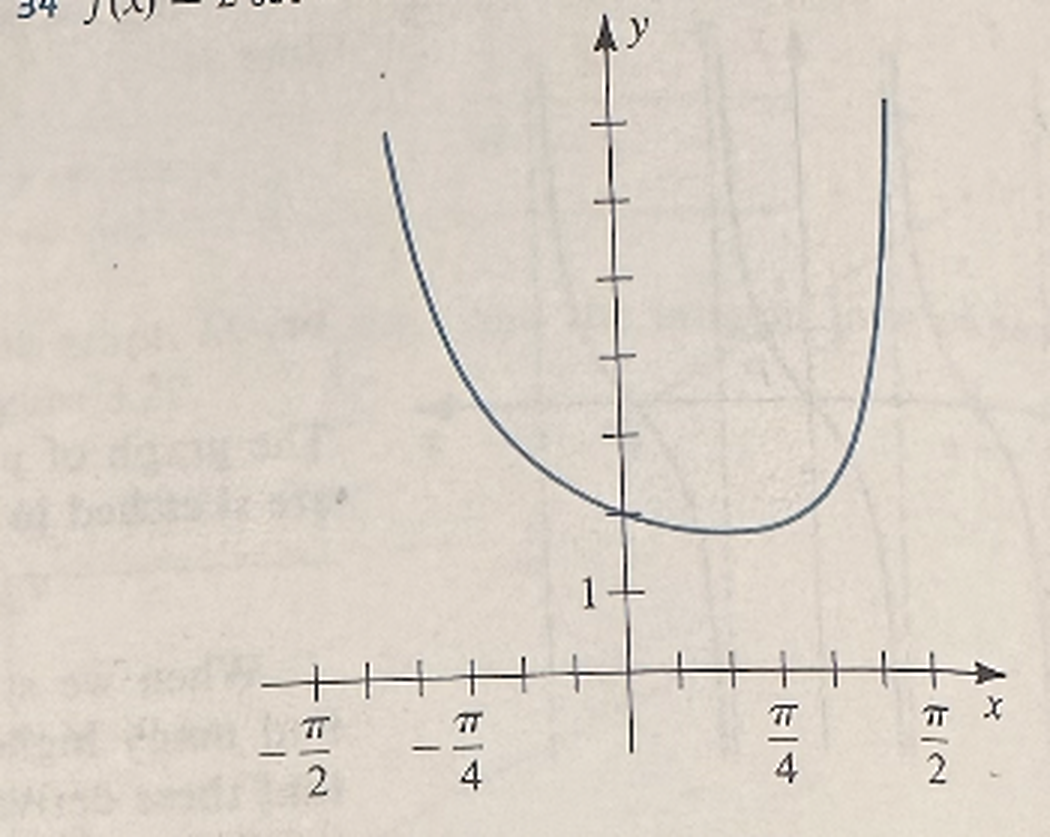
\includegraphics[width=0.5\linewidth]{fig-3.4-3.9-q10.png}
  \wsG
\end{probs}

\begin{probs}
  \prob{11} If $y=1+2\cos x$, find
  \begin{enumerate}[label=\textbf{(\alph*)},leftmargin=2.4em,itemsep=4pt,topsep=4pt]
    \item the $x$-coordinates of all points on the graph at which the tangent line is
          perpendicular to the line $y=\dfrac{1}{\sqrt{3}}x+4$ \wsM
    \item an equation of the tangent line to the graph at the point where the graph
          crosses the $y$-axis \wsM
  \end{enumerate}
\end{probs}

\headnote{(a) Find equations of the tangent line and the normal line to the graph of the
equation at $P$. \ (b) Find the $x$-coordinates on the graph at which the tangent line is
horizontal.}
\begin{probs}
  \prob{12} $y=\left(x+\dfrac{1}{x}\right)^{5};\qquad P(1,32)$ \wsL
\end{probs}

\begin{probs}
  \prob{13} If $k(x)=f(g(x))$ and if $f(2)=-4$, $g(2)=2$, $f'(2)=3$, and $g'(2)=5$,
            find $k(2)$ and $k'(2)$. \wsM
\end{probs}

\clearpage

\headnote{Multiple choice. No calculator unless a problem says otherwise.}
\begin{probs}
  \prob{14} If $y=\sin x$ and $y^{(n)}$ means ``the $n$th derivative of $y$ with respect
            to $x$,'' then the smallest positive integer $n$ for which $y^{(n)}=y$ is
  \mc{$2$}{$4$}{$5$}{$6$}{$8$}
  \wsS

  \prob{15} $\displaystyle\lim_{h\to0}\frac{\sin(x+h)-\sin x}{h}$ is
  \mc{$0$}{$1$}{$\sin x$}{$\cos x$}{nonexistent}
  \wsS

  \prob{16} If $f(x)=\dfrac{x}{\tan x}$, then $f'\!\left(\dfrac{\pi}{4}\right)=$
  \mc{$2$}{$\dfrac{1}{2}$}{$1+\dfrac{\pi}{2}$}{$\dfrac{\pi}{2}-1$}{$1-\dfrac{\pi}{2}$}
  \wsM

  \prob{17} The graph of the function $f$ shown below has a vertical tangent at the point
            $(2,0)$ and horizontal tangents at the points $(1,-1)$ and $(3,1)$.
            For what values of $x$, $-2<x<4$, is $f$ \emph{not} differentiable?

  \smallskip
  \noindent\includegraphics[width=0.52\linewidth]{fig-3.4-3.9-q17.png}

  \mc{$0$ only}{$0$ and $2$ only}{$1$ and $3$ only}{$0$, $1$, and $3$ only}{$0$, $1$, $2$, and $3$}
  \wsG

  \prob{18} The value of the derivative of $y=\dfrac{\sqrt[3]{x^{2}+8}}{\sqrt[4]{2x+1}}$
            at $x=0$ is \quad \textit{(calculator permitted)}
  \mc{$-1$}{$-\dfrac{1}{2}$}{$0$}{$\dfrac{1}{2}$}{$1$}
  \wsM

  \prob{19} The line normal to the curve $y=\sqrt{16-x}$ at the point $(0,4)$ has slope
  \mc{$8$}{$4$}{$\dfrac{1}{8}$}{$-\dfrac{1}{8}$}{$-8$}
  \wsM

  \prob{20} If $f$ and $g$ are twice differentiable and if $h(x)=f(g(x))$, then $h''(x)=$
  \begin{enumerate}[label=\textbf{(\Alph*)},leftmargin=2.4em,itemsep=3pt,topsep=4pt]
    \item $f''(g(x))\bigl[g'(x)\bigr]^{2}+f'(g(x))g''(x)$
    \item $f''(g(x))g'(x)+f'(g(x))g''(x)$
    \item $f''(g(x))\bigl[g'(x)\bigr]^{2}$
    \item $f''(g(x))g''(x)$
    \item $f''(g(x))$
  \end{enumerate}
  \wsM

  \prob{21} If $h(x)=f^{2}(x)-g^{2}(x)$, $f'(x)=-g(x)$, and $g'(x)=f(x)$, then $h'(x)=$
  \mc{$0$}{$1$}{$-4f(x)g(x)$}{$\bigl(-g(x)\bigr)^{2}-\bigl(f(x)\bigr)^{2}$}{$-2\bigl(-g(x)+f(x)\bigr)$}
  \wsM

  \prob{22} Let $f$ and $g$ be differentiable functions such that
  \[
    f(1)=2,\qquad f'(1)=3,\qquad f'(2)=-4,
  \]
  \[
    g(1)=2,\qquad g'(1)=-3,\qquad g'(2)=5.
  \]
  If $h(x)=f(g(x))$, then $h'(1)=$
  \mc{$-9$}{$-4$}{$0$}{$12$}{$15$}
  \wsM
\end{probs}

\clearpage
%======================================================================
\section*{Tommy's Questions}
\noindent\textit{These two are written by us. Each one pulls several ideas together at once,
so show all of your work.}
\medskip

\noindent\textbf{Tommy 1.}\quad Let $f(x)=x+2\sin x$ on the interval $[0,2\pi]$.
\begin{enumerate}[label=\textbf{(\alph*)},leftmargin=2.8em,itemsep=6pt,topsep=5pt]
  \item Find $f'(x)$. \wsS
  \item Find every $x$ in $[0,2\pi]$ at which the tangent line to the graph of $f$ is
        horizontal. \wsM
  \item Find every $x$ in $[0,2\pi]$ at which the tangent line to the graph of $f$ is
        \emph{perpendicular} to the line $x+y=5$.
        \textit{(Careful: perpendicular, not parallel.)} \wsM
  \item Write an equation of the tangent line to the graph of $f$ at the point where the
        graph crosses the $y$-axis. \wsM
\end{enumerate}

\bigskip
\noindent\textbf{Tommy 2.}\quad Let $y$ be the positive function defined, for $x$ near
$\dfrac{\pi}{3}$, by the infinitely nested radical
\[
  y=\sqrt{\,\sec x+\sqrt{\,\sec x+\sqrt{\,\sec x+\sqrt{\cdots}}}}\;,
\]
which you may assume converges. Find the \textbf{exact} value of $\dfrac{dy}{dx}$ at
$x=\dfrac{\pi}{3}$.
\wsL
\wsL

\bigskip
\noindent\textbf{Tommy 3.}\quad Let
\[
  f(x)=\frac{x}{\sqrt{1+x^{2}}}\,,
\]
and for each positive integer $n$ let $f_{n}$ denote $f$ composed with itself $n$ times, so
that $f_{1}(x)=f(x)$, \ $f_{2}(x)=f(f(x))$, \ $f_{3}(x)=f(f(f(x)))$, and so on.
Find the \textbf{exact} value of $f_{100}'(1)$.
\wsL
\wsL

\clearpage
%======================================================================
\begin{center}\Large\textbf{Answer Key}\end{center}
\medskip
\noindent\textit{Answers only for 1--22. Tommy's questions are worked in full.}
\medskip

\begin{multicols}{2}
\begin{ans}
  \ansitem{1} $-4\sin x$
  \ansitem{2} $\dfrac{\theta\cos\theta-\sin\theta}{\theta^{2}}$
  \ansitem{3} $17000\,(17v-5)^{999}$
  \ansitem{4} $-4\csc^{2}2\phi\,\cot 2\phi$
  \ansitem{5} $\dfrac{4\sin\!\left(2\sqrt{3-8\theta}\right)}{\sqrt{3-8\theta}}$
  \ansitem{6} $\dfrac{3}{\sqrt{6t+5}}$
  \ansitem{7} $\dfrac{1024\,s\,(2s^{2}-1)^{3}(18s^{3}-27s+4)}{(1-9s^{3})^{5}}$
  \ansitem{8} $\dfrac{1}{z^{2}}\csc\!\left(\dfrac{1}{z}\right)\cot\!\left(\dfrac{1}{z}\right)-\sin z$
  \ansitem{9} $10\sec^{2}(5x)\tan(5x)$
  \ansitem{10} $\left(\dfrac{\pi}{6},\ \sqrt{3}\right)$
  \ansitem{11} (a) $x=\dfrac{\pi}{3}+2\pi n$ and $x=\dfrac{2\pi}{3}+2\pi n$, $n$ any
               integer \ \ (b) $y=3$
  \ansitem{12} (a) tangent $y=32$; \ normal $x=1$ \ \ (b) $x=-1$ and $x=1$
  \ansitem{13} $k(2)=-4$, \ $k'(2)=15$
  \ansitem{14} (B)
  \ansitem{15} (D)
  \ansitem{16} (E)
  \ansitem{17} (B)
  \ansitem{18} (A)
  \ansitem{19} (A)
  \ansitem{20} (A)
  \ansitem{21} (C)
  \ansitem{22} (D)
\end{ans}
\end{multicols}

\bigskip
\noindent\textbf{Tommy 1.}\quad $f(x)=x+2\sin x$ on $[0,2\pi]$.
\begin{enumerate}[label=\textbf{(\alph*)},leftmargin=2.8em,itemsep=6pt,topsep=5pt]
  \item $f'(x)=1+2\cos x$.

  \item Horizontal tangent means $f'(x)=0$:
        \[
          1+2\cos x=0 \ \Longrightarrow\ \cos x=-\tfrac{1}{2}
          \ \Longrightarrow\ x=\frac{2\pi}{3},\ \frac{4\pi}{3}.
        \]
        Both lie in $[0,2\pi]$, so both count.

  \item $x+y=5$ has slope $-1$. A line perpendicular to it has slope
        $-\dfrac{1}{-1}=1$ --- \emph{not} $-1$. So set $f'(x)=1$:
        \[
          1+2\cos x=1 \ \Longrightarrow\ \cos x=0
          \ \Longrightarrow\ x=\frac{\pi}{2},\ \frac{3\pi}{2}.
        \]

  \item The graph crosses the $y$-axis at $x=0$: $f(0)=0+2\sin 0=0$, so the point is
        $(0,0)$. The slope there is $f'(0)=1+2\cos 0=3$. The tangent line is
        \[
          y-0=3(x-0),\qquad\text{that is,}\qquad y=3x.
        \]
\end{enumerate}

\bigskip
\noindent\textbf{Tommy 2.}\quad Answer: $\dfrac{dy}{dx}\bigg|_{x=\pi/3}=\dfrac{2\sqrt{3}}{3}$.

\medskip
\noindent\textbf{The way in.} Look at what sits under the outermost radical: it is
$\sec x$ plus \emph{the entire original expression again}. The tail is a copy of the whole
thing, so it equals $y$:
\[
  y=\sqrt{\sec x+y}\,,\qquad\text{and squaring,}\qquad y^{2}=\sec x+y .
\]
That one line replaces an infinite tower with a single equation. There is nothing left to
differentiate layer by layer.

\medskip
\noindent\textbf{Differentiate implicitly.} Both sides with respect to $x$, remembering that
$y$ is a function of $x$ (so $y^{2}$ needs the chain rule, giving $2y\,y'$, not $2y$):
\[
  2y\,\frac{dy}{dx}=\sec x\tan x+\frac{dy}{dx}
  \qquad\Longrightarrow\qquad
  \frac{dy}{dx}\,(2y-1)=\sec x\tan x
  \qquad\Longrightarrow\qquad
  \frac{dy}{dx}=\frac{\sec x\tan x}{2y-1}.
\]

\medskip
\noindent\textbf{Find $y$ at $x=\pi/3$.} Since $\sec\dfrac{\pi}{3}=2$, the equation
$y^{2}=\sec x+y$ becomes
\[
  y^{2}-y-2=0,\qquad (y-2)(y+1)=0,\qquad y=2\ \text{ or }\ y=-1 .
\]
A square root is never negative, so $y=2$ and the root $y=-1$ is discarded.

\medskip
\noindent\textbf{Evaluate.} With $\sec\dfrac{\pi}{3}=2$ and $\tan\dfrac{\pi}{3}=\sqrt{3}$,
\[
  \left.\frac{dy}{dx}\right|_{x=\pi/3}
  =\frac{(2)\bigl(\sqrt{3}\bigr)}{2(2)-1}
  =\frac{2\sqrt{3}}{3}\;\approx\;1.1547 .
\]

\medskip
\noindent\textbf{Check it the long way.} Solving $y^{2}-y-\sec x=0$ outright gives
$y=\dfrac{1+\sqrt{1+4\sec x}}{2}$, and differentiating \emph{that} directly gives
$\dfrac{dy}{dx}=\dfrac{\sec x\tan x}{\sqrt{1+4\sec x}}$, which at $x=\dfrac{\pi}{3}$ is
$\dfrac{2\sqrt{3}}{\sqrt{9}}=\dfrac{2\sqrt{3}}{3}$. Same answer, more algebra.

\medskip
\noindent\textbf{The two traps.} Keeping $y=-1$ --- it solves the quadratic but not the
original problem, because the radical is positive. And peeling the radicals one layer at a
time, which never terminates: the whole point is that the tower is self-similar.

\bigskip
\noindent\textbf{Tommy 3.}\quad Answer:
$f_{100}'(1)=\dfrac{1}{101\sqrt{101}}=\dfrac{\sqrt{101}}{10201}\approx 0.000985$.

\medskip
\noindent\textbf{The way in.} Do not differentiate anything yet --- compose twice and watch
what happens. Substituting $f(x)$ into $f$,
\[
  f_{2}(x)=f\bigl(f(x)\bigr)
  =\frac{\dfrac{x}{\sqrt{1+x^{2}}}}{\sqrt{1+\dfrac{x^{2}}{1+x^{2}}}}\,.
\]
The radical in the denominator simplifies first:
$1+\dfrac{x^{2}}{1+x^{2}}=\dfrac{1+2x^{2}}{1+x^{2}}$, so
\[
  f_{2}(x)=\frac{x}{\sqrt{1+x^{2}}}\cdot\frac{\sqrt{1+x^{2}}}{\sqrt{1+2x^{2}}}
          =\frac{x}{\sqrt{1+2x^{2}}}\,.
\]
The $\sqrt{1+x^{2}}$ cancels completely. Running the same computation again gives
$f_{3}(x)=\dfrac{x}{\sqrt{1+3x^{2}}}$, and the pattern is
\[
  \boxed{\,f_{n}(x)=\frac{x}{\sqrt{1+nx^{2}}}\,}
\]
Composing $f$ with itself does nothing but advance the counter under the radical. In
particular $f_{100}(x)=\dfrac{x}{\sqrt{1+100x^{2}}}$ --- and now there is one function to
differentiate instead of one hundred.

\medskip
\noindent\textbf{Differentiate.} Write $f_{100}(x)=x\bigl(1+100x^{2}\bigr)^{-1/2}$ and use the
product rule with the chain rule:
\[
  f_{100}'(x)=\bigl(1+100x^{2}\bigr)^{-1/2}
             +x\cdot\left(-\tfrac{1}{2}\right)\bigl(1+100x^{2}\bigr)^{-3/2}(200x)
            =\bigl(1+100x^{2}\bigr)^{-1/2}-100x^{2}\bigl(1+100x^{2}\bigr)^{-3/2}.
\]
Factor out $\bigl(1+100x^{2}\bigr)^{-3/2}$ and the bracket collapses:
\[
  f_{100}'(x)=\bigl(1+100x^{2}\bigr)^{-3/2}\Bigl[\bigl(1+100x^{2}\bigr)-100x^{2}\Bigr]
             =\bigl(1+100x^{2}\bigr)^{-3/2}.
\]
(The same thing happens for every $n$: $f_{n}'(x)=\bigl(1+nx^{2}\bigr)^{-3/2}$, because the
bracket is always exactly $1$.)

\medskip
\noindent\textbf{Evaluate at $x=1$.}
\[
  f_{100}'(1)=(1+100)^{-3/2}=101^{-3/2}=\frac{1}{101\sqrt{101}}
             =\frac{\sqrt{101}}{10201}.
\]

\medskip
\noindent\textbf{The trap.} Reaching straight for the chain rule. Writing
$f_{100}'(1)=f'\bigl(f_{99}(1)\bigr)\cdot f'\bigl(f_{98}(1)\bigr)\cdots f'(1)$ is perfectly
correct and perfectly useless --- it is a product of one hundred factors you cannot evaluate.
The composition has to be \emph{simplified} before it is differentiated.

\clearpage
% === SOURCELIST ===
%======================================================================
\begin{center}\Large\textbf{Where These Questions Came From}\end{center}
\medskip

\noindent These questions come from Sections 3.4, 3.6 and the Chapter 3 Review Exercises
of the textbook, plus two pages of the AP packet. If you got one wrong, look it up and try
the problems around it --- that is where the extra practice is.
\medskip

\begin{multicols}{2}
\noindent\textbf{Section 3.4}
\begin{itemize}[leftmargin=1.6em,itemsep=1pt,topsep=2pt]
  \item[] \textbf{1} $=$ 3.4 \#1
  \item[] \textbf{2} $=$ 3.4 \#7
  \item[] \textbf{10} $=$ 3.4 \#34
  \item[] \textbf{11} $=$ 3.4 \#38
\end{itemize}

\smallskip
\noindent\textbf{Section 3.6}
\begin{itemize}[leftmargin=1.6em,itemsep=1pt,topsep=2pt]
  \item[] \textbf{3} $=$ 3.6 \#15
  \item[] \textbf{4} $=$ 3.6 \#39
  \item[] \textbf{5} $=$ 3.6 \#55
  \item[] \textbf{12} $=$ 3.6 \#65
  \item[] \textbf{13} $=$ 3.6 \#81
\end{itemize}

\smallskip
\noindent\textbf{Chapter 3 Review Exercises (3.9)}
\begin{itemize}[leftmargin=1.6em,itemsep=1pt,topsep=2pt]
  \item[] \textbf{6} $=$ 3.9 \#5
  \item[] \textbf{7} $=$ 3.9 \#15
  \item[] \textbf{8} $=$ 3.9 \#26
  \item[] \textbf{9} $=$ 3.9 \#39
\end{itemize}

\smallskip
\noindent\textbf{AP Packet page 5}
\begin{itemize}[leftmargin=1.6em,itemsep=1pt,topsep=2pt]
  \item[] \textbf{14} $=$ BC 8 (1973)
  \item[] \textbf{15} $=$ BC 10 (1988)
  \item[] \textbf{16} $=$ BC 6 (1985)
  \item[] \textbf{17} $=$ BC 13 (1988)
\end{itemize}

\smallskip
\noindent\textbf{AP Packet page 7}
\begin{itemize}[leftmargin=1.6em,itemsep=1pt,topsep=2pt]
  \item[] \textbf{18} $=$ BC 21 (1993)
  \item[] \textbf{19} $=$ BC 6 (1997)
  \item[] \textbf{20} $=$ BC 5 (1998)
  \item[] \textbf{21} $=$ BC 8 (1969)
  \item[] \textbf{22} $=$ BC 39 (1973)
\end{itemize}

\smallskip
\noindent\textbf{Tommy's Questions}
\begin{itemize}[leftmargin=1.6em,itemsep=1pt,topsep=2pt]
  \item[] \textbf{Tommy 1} --- original, not in the textbook
  \item[] \textbf{Tommy 2} --- original, not in the textbook
  \item[] \textbf{Tommy 3} --- original, not in the textbook
\end{itemize}
\end{multicols}

\end{document}
